\section{Funzionalità}
Tutte le seguenti funzionalità sono disponibili solo dopo aver selezionato un
dataset\textsubscript{g}, atteso il caricamento e raggiunto l'ambiente 3D.

\subsection{Visualizzazione tooltip}
Il tooltip\textsubscript{g} è un elemento grafico che fornisce informazioni aggiuntive su un
particolare elemento del grafico. Quando l'utente passa il mouse su una barra\textsubscript{g}
del grafico, viene visualizzato un tooltip\textsubscript{g} che mostra il valore associato a
quella barra\textsubscript{g}, nonché le etichette ad essa associate.
\begin{figure}[ht!]
    \centering
    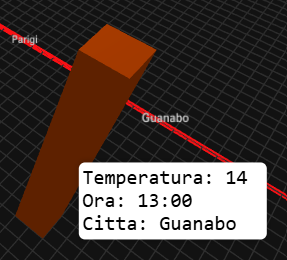
\includegraphics[scale=0.6]{template/images/tooltip.png}
    \caption{Tooltip\textsubscript{g}}
\end{figure}

\subsection{Navigazione 3D}
All'interno dell'ambiente 3D l'utente può interagire con il grafico con le
seguenti modalità:
\begin{itemize}
    \item \textbf{Spostamento:} l'utente può spostare il grafico senza cambiarne
          l'angolazione tenendo premuto il tasto destro del mouse e trascinando
          nella direzione desiderata;
    \item \textbf{Zoom:} l'utente può ingrandire o ridurre il grafico
          utilizzando la rotellina del mouse o il gesto di pinch\textsubscript{g} sul touchpad;
    \item \textbf{Rotazione:} l'utente può ruotare il grafico senza spostarlo
          tenendo premuto il tasto sinistro del mouse e trascinando nella direzione desiderata;
\end{itemize}
Questi controlli sono sempre attivi quando il cursore è sopra il grafico.
\begin{figure}[ht!]
    \centering
    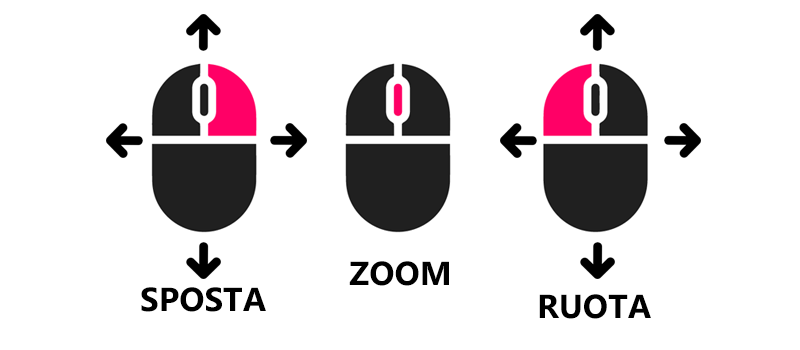
\includegraphics[scale=0.6]{template/images/comandi.png}
    \caption{Comandi per la navigazione}
\end{figure}

\subsection{Navigazione avanzata}
L'utente può usufruire di funzionalità avanzate per la navigazione del grafico
3D\textsubscript{g}:
\begin{itemize}
    \item \textbf{Rotazione tramite gizmo\textsubscript{g}:} l'utente può ruotare il grafico
          senza spostarlo tenendo premuto il tasto sinistro del mouse su un'estremità
          dell'asse del gizmo\textsubscript{g} e trascinando nella direzione desiderata;
    \item \textbf{Reset:} l'utente può riportare il grafico alla posizione
          iniziale premendo il pulsante di reset della
          visualizzazione in alto a sinistra, sotto al gizmo\textsubscript{g}.
\end{itemize}
\begin{figure}[ht!]
    \centering
    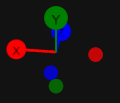
\includegraphics[scale=0.6]{template/images/gizmo.png}
    \hspace{1cm}
    
\includegraphics[scale=0.6]{template/images/resetcam.png}
    \caption{Elementi per la navigazione avanzata}
\end{figure}

\subsection{Filtraggio dei dati}
L'utente può filtrare i dati che soddisfano certe proprietà. Nel grafico 3D\textsubscript{g}, i
dati filtrati vengono visualizzati con la massima opacità, mentre i dati non
filtrati vengono visualizzati con un'opacità ridotta. Nella tabella, le celle
che contengono i dati filtrati hanno sfondo verde, mentre quelle che contengono
i dati non filtrati hanno sfondo grigio. \\ Il filtraggio dei dati può essere
eseguito in base a tre criteri:
\begin{itemize}
    \item \textbf{Valore medio\textsubscript{g}:} l'utente può filtrare i dati in base al valore
          medio\textsubscript{g} del dataset\textsubscript{g}, che viene calcolato automaticamente. L'utente può
          scegliere di visualizzare solo i valori superiori o inferiori al valore
          medio\textsubscript{g}, selezionando l'opzione desiderata sotto la voce "SCEGLI
          L'ALGORITMO DI FILTRAGGIO". Per accedere a questa funzionalità, l'utente
          deve premere il pulsante "Filtra" situato nel
          form delle opzioni, sotto la voce "FILTRA PER VALOR MEDIO GLOBALE";
    \item \textbf{Valore del dataset\textsubscript{g}:} l'utente può filtrare i dati in base a un
          valore del dataset\textsubscript{g}. L'utente
          può scegliere di visualizzare solo i valori superiori o inferiori al
          valore di riferimento, selezionando l'opzione desiderata sotto la voce
          "SCEGLI L'ALGORITMO DI FILTRAGGIO". Per accedere a questa funzionalità,
          l'utente deve cliccare sulla barra\textsubscript{g} del grafico o sulla cella della tabella che contiene il
          valore desiderato;
    \item \textbf{Primi N valori:} l'utente può filtrare i dati in base ai primi N
          valori più alti o più bassi del dataset\textsubscript{g}, dove il numero N deve essere un intero positivo
          inserito dall'utente nel campo di input del form delle opzioni. Se il numero inserito supera il numero totale di valori
          del dataset\textsubscript{g}, verranno filtrati tutti i dati. L'utente può scegliere di visualizzare solo i valori
          più alti o più bassi al valore di riferimento, selezionando l'opzione
          desiderata sotto la voce "SCEGLI L'ALGORITMO DI FILTRAGGIO". Per accedere a questa funzionalità,
          l'utente deve premere il pulsante "Filtra" situato nel form delle
          opzioni, sotto la voce "FILTRA I PRIMI N VALORI".
\end{itemize}
Per rimuovere il filtro applicato, l'utente deve premere il pulsante "Resetta filtri" nel form delle opzioni.
\begin{figure}[H]
    \centering
    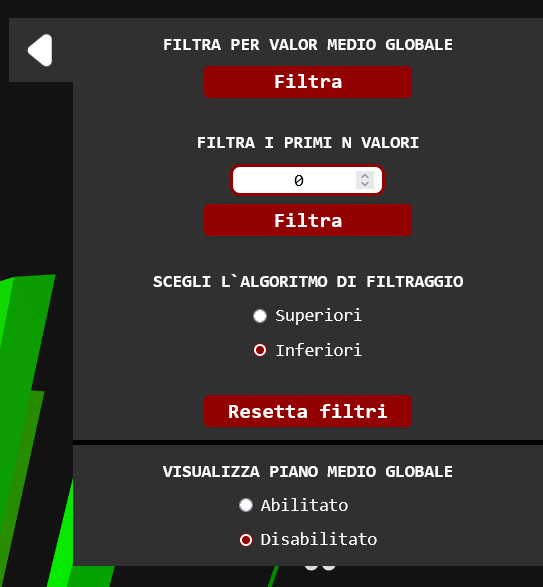
\includegraphics[scale=0.6]{template/images/env/options.png}
    \caption{Form delle opzioni}
\end{figure}

\subsection{Visualizzazione del piano medio}
L'utente può visualizzare il piano medio, ovvero il piano parallelo al
piano XZ (base del grafico), situato all'altezza del valore medio\textsubscript{g} del dataset\textsubscript{g}.
Per rendere tale piano visibile, l'utente deve selezionare l'opzione "Abilitato" sotto la voce
"VISUALIZZA PIANO MEDIO GLOBALE" nel form delle opzioni. Analogamente, per
nasconderlo, l'utente deve selezionare l'opzione "Disabilitato".
\begin{figure}[H]
    \centering
    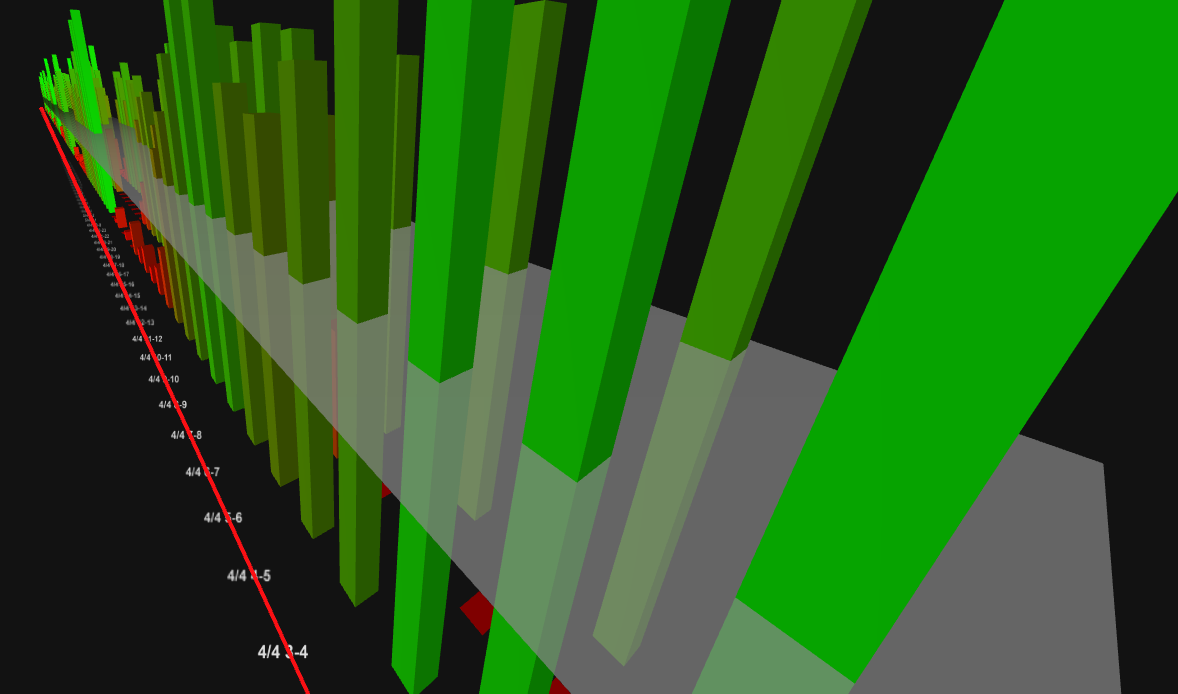
\includegraphics[scale=0.45]{template/images/env/plane.png}
    \caption{Piano medio del dataset\textsubscript{g}}
\end{figure}

\subsection{Autoposizionamento}
L'utente può posizionare il grafico in modo che una barra\textsubscript{g} specifica risulti
visibile e non completamente nascosta dalle altre barre\textsubscript{g}. 
Per farlo, l'utente deve cliccare sulla barra\textsubscript{g} del grafico o sulla
cella della tabella che contiene il valore desiderato. Inoltre, la barra\textsubscript{g}
selezionata assume il colore bianco.
\begin{figure}[ht!]
    \centering
    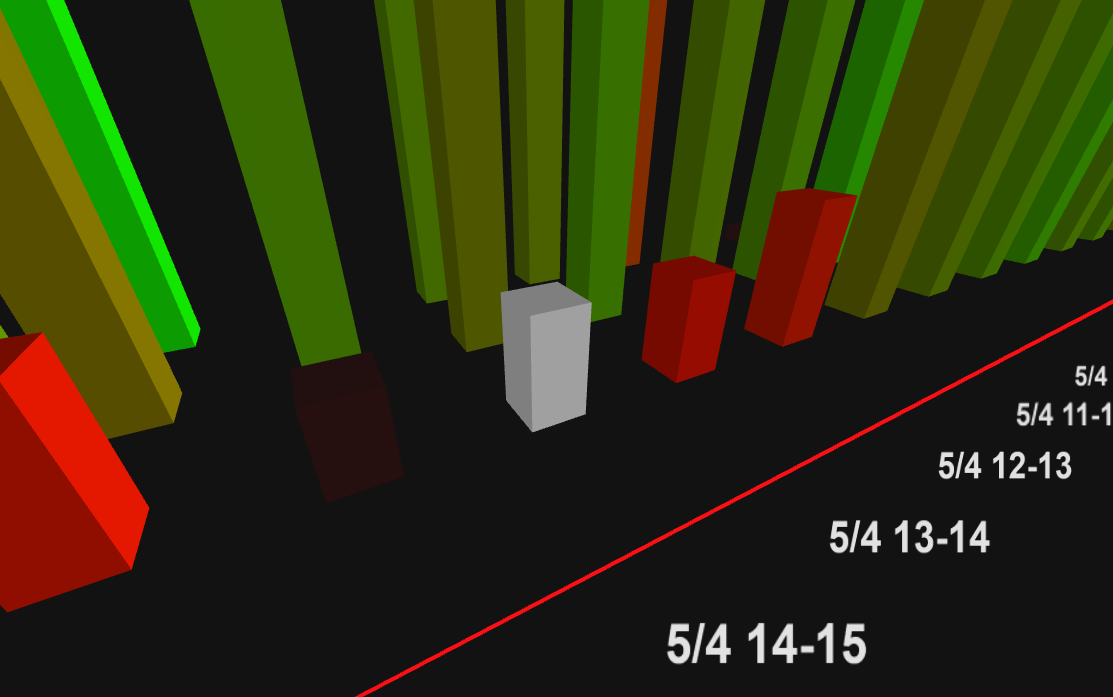
\includegraphics[scale=0.45]{template/images/env/autofocus.png}
    \caption{Grafico con barra\textsubscript{g} selezionata}
\end{figure}